\chapter{Background}

\section{The sandeel}
    

\section{The sandeel survey and acoustic data} \label{acoustic_data}
    things


\section{Machine Learning} \label{Machine Learning}
    As described in the book Deep Learning\cite{Goodfellow-et-al-2016_ML} machine learning can intuitively be split into four parts; The algorithm, empirical data, a task and a performance measure. A machine learning algorithm can then be identified as an algorithm that increases its performance on a task, given data. As this happens, the algorithm is said to be learning. The task itself and the data the algorithm is given may vary. This is why we can approximately divide the machine learning approaches into three categories\cite{Goodfellow-et-al-2016_E}: supervised learning, unsupervised and reinforcement learning. 
    
    \subsection{Algorithm types} \label{Algorithm types}
        \subsubsection{Supervised learning}
            Supervised learning \cite{Goodfellow-et-al-2016_E} algorithms base themselves on datasets containing samples that also have a label. This means the output the algorithm will have to predict. These labels can for example be binary class or consist of a multitude of classes or values in regression problems.
            
        \subsubsection{Unsupervised learning}
            Unlike supervised leaning, the unsupervised learning \cite{Goodfellow-et-al-2016_E} algorithms only have the data and will learn properties contained in the data. A practical example is clustering, where you can divide a dataset into clusters based on similar features. 
                
        \subsubsection{Reinforcement learning}
            In reinforcement learning \cite{Goodfellow-et-al-2016_E}, the algorithm do not learn from a given dataset, but will act in an environment. In some cases this is a feedback loop giving either a positive or negative reward for performing certain actions. The goal is then for the algorithm to maximize this reward. This is what people often associate with \gls{ai} and can be for example seen in the AlphaZero software that beat professional chess players\cite{silver2017mastering}.
    
    \subsection{Data}
        things
    \subsection{Features}
        things
    \subsection{Overfitting vs. underfitting}
        things
    \subsection{Bias - variance tradeoff}
        things
    \subsection{Model evaluation}
        things
    \subsubsection{Train-Val-Test split}
        things
    \subsubsection{F1-score, Precision, Recall} \label{f1_score}
        things
    \subsubsection{Hyperparameter-search}
        things

\section{Artificial Neural Networks} \label{neural networks}
    \citeauthor{Goodfellow-et-al-2016_NN} \cite{Goodfellow-et-al-2016_NN} describes \gls{ann} as a unknown function \textit{\^{f}} that maps an input \textit{x} to an output \textit{y}. The goal is then to approximate some optimal function \textit{f} through learning from examples. In this section, I will explain the basics of \gls{ann}s.

    \subsection{Perceptron} \label{perceptron}
        The \gls{ann}s fundamental building block is called an artificial neuron or perceptron. It is formulated in the following way\cite{razavi2021deep_exp_per}:
            \begin{equation} \label{eq_perceptron}
                y = \sigma(\sum_{i=1}^{D}w_ix_i + b)
            \end{equation}
            
        where D is the number dimension of the input space, x is the input vector and w is a set of weights that is of the same size as x, b is the bias and {\textsigma} is a nonlinear activation function which will be explained later in \ref{activation function}. In short the equation inside the activation functions is a linear regression. The perceptron is illustrated in figure \ref{Perceptron / MLP}.
    
    \subsection{Multi-layered perceptron} \label{MLP}
        The neurons presented in section \ref{perceptron} are then piled together in layers to form a \gls{ann}, which in turn forms what is called a \gls{mlp} \cite{razavi2021deep_exp_per}. All the neurons in each layer are connected to every neuron in the next layer, as depicted in figure \ref{Perceptron / MLP}.
        
            \begin{figure}[H]
                \centering
                \includegraphics[scale=0.5]{figures/perceptron.png}
                \caption{(a) A perceptron and (b) a multi-layer perceptron with four inputs in the input-layer(arrows to the left), two hidden layers(green), and three outputs in the output-layer(red).}
              	\medskip 
                \hspace*{15pt}\hbox{\scriptsize Credit: \citeauthor{razavi2021deep_exp_DL}\cite{razavi2021deep_exp_DL}}
                \label{Perceptron / MLP}
            \end{figure}
        
        The architecture of the \gls{ann} consist of an input layer, a user defined number of hidden layers and finally an output layer. A \gls{mlp} is a type of network called feed-forward \gls{ann} because the data flows from the input to the output layer. The parameters that are adjusted through training (explained in section XXX) are all the weights between every neuron in the network and the individual biases. The intuition for the MLP depicted in \ref{Perceptron / MLP} is that different neurons will fire with varying strengths depending on the input, resulting in different outputs.
        
    \subsection{Activation function} \label{activation function}
        The activations function is what enables the \gls{ann} to learn non-linear features \cite{razavi2021deep_exp_per}. The reason you need it is that a network consisting of only linear layers will just be the same as a single linear layer \cite{razavi2021deep_exp_per}. The activation function used in this thesis was the ReLU which stands for rectified as described in \cite{sharma2019new_activation_func}. The formula for it is as follows:
            \begin{equation} \label{relu_eq}
                f(x) = max(0,x)
            \end{equation}
        As can be seen in figure \ref{activation_fig} the function is 0 while x is less than 0 and then linear. Intuitively, this function can make a selection of neurons in figure \ref{MLP} send their computed value forth, and some  other neurons output nothing. This can result in greater efficiency and faster training, as not all neurons are active \cite{sharma2019new_activation_func}.
        
        An example of another activation function is the sigmoid \cite{sharma2019new_activation_func}, which transforms the values in the range 0 to 1. I will list the formula and have included it in the plot \ref{activation_fig}, but will not go any further as it is not necessary for understanding this thesis. Sigmoid formula:
            \begin{equation} \label{sigmoid_eq}
                f(x) = \dfrac{1}{e^{-x}} 
            \end{equation}
            
            \begin{figure}[H]
                \centering
                \includegraphics[scale=0.5]{figures/activation.png}
                \caption{A ReLU function (blue) and a sigmoid function (red)}.
              	\medskip 
                \label{activation_fig}
            \end{figure}

\section{Training Neural Networks} \label{training neural networks}
    thing
\subsection{Backpropagation}
    things
\subsection{Gradient Decent}
    things
\subsection{Batch learning}
    things
\subsection{Regularization}
    things
\subsection{Batch-Norm}
    things
\subsection{Data-Augmentation}
    things

\section{Computer vision}
    things
\subsection{Convolutional neural network}
    \gls{cnn} are a type of \gls{ann}s that are primarily used in machine learning tasks concerning images\cite{o2015introduction_convolutions}. The \gls{cnn} is built around an operation called convolutions that \textit{convolutes} over its input, hence the name. Unlike the regular neurons that has a connection to every neuron in the previous layer, in the convolution operation, every neuron consists of a weight matrix of three dimensions; \textit{height}, \textit{width} and \textit{depth}. The depth is the size of the third dimension of the input, like the three colors in standard images. This creates what is called a \textit{filter} which is applied to the input in what is defined as \textit{strides}, and calculates the scalar product between the weights and the connected area of the input. The complete convolutional operations then consist of applying this filter to the entire input. This reduces the dimension of the input to a 2D output, but you may apply several filters to increase the dimensions, as each will create a new 2D channel in the output. Reductions in the height and width will normally occur with the standard convolutions, and this type is called \textit{valid convolutions}. Later in this section \textit{same convolutions} will be described which conserves the input dimensions. The high level convolutional operation is illustrated in figure \ref{convolutional_filters_fig}. A more detailed example can be found in figure \ref{convolutional_fig} which looks at how a convolution is applied to 2D input. 
    
    \begin{figure}[H]
        \centering
        \includegraphics[scale=0.5]{figures/convolution.png}
        \caption{The yellow outline in the input illustrated where the filter is applied. This produces a single value. More filters could be added to increase the dimension of the output.}
      	\medskip 
        \label{convolutional_filters_fig}
    \end{figure}
    

    
    \begin{figure}[H]
        \centering
        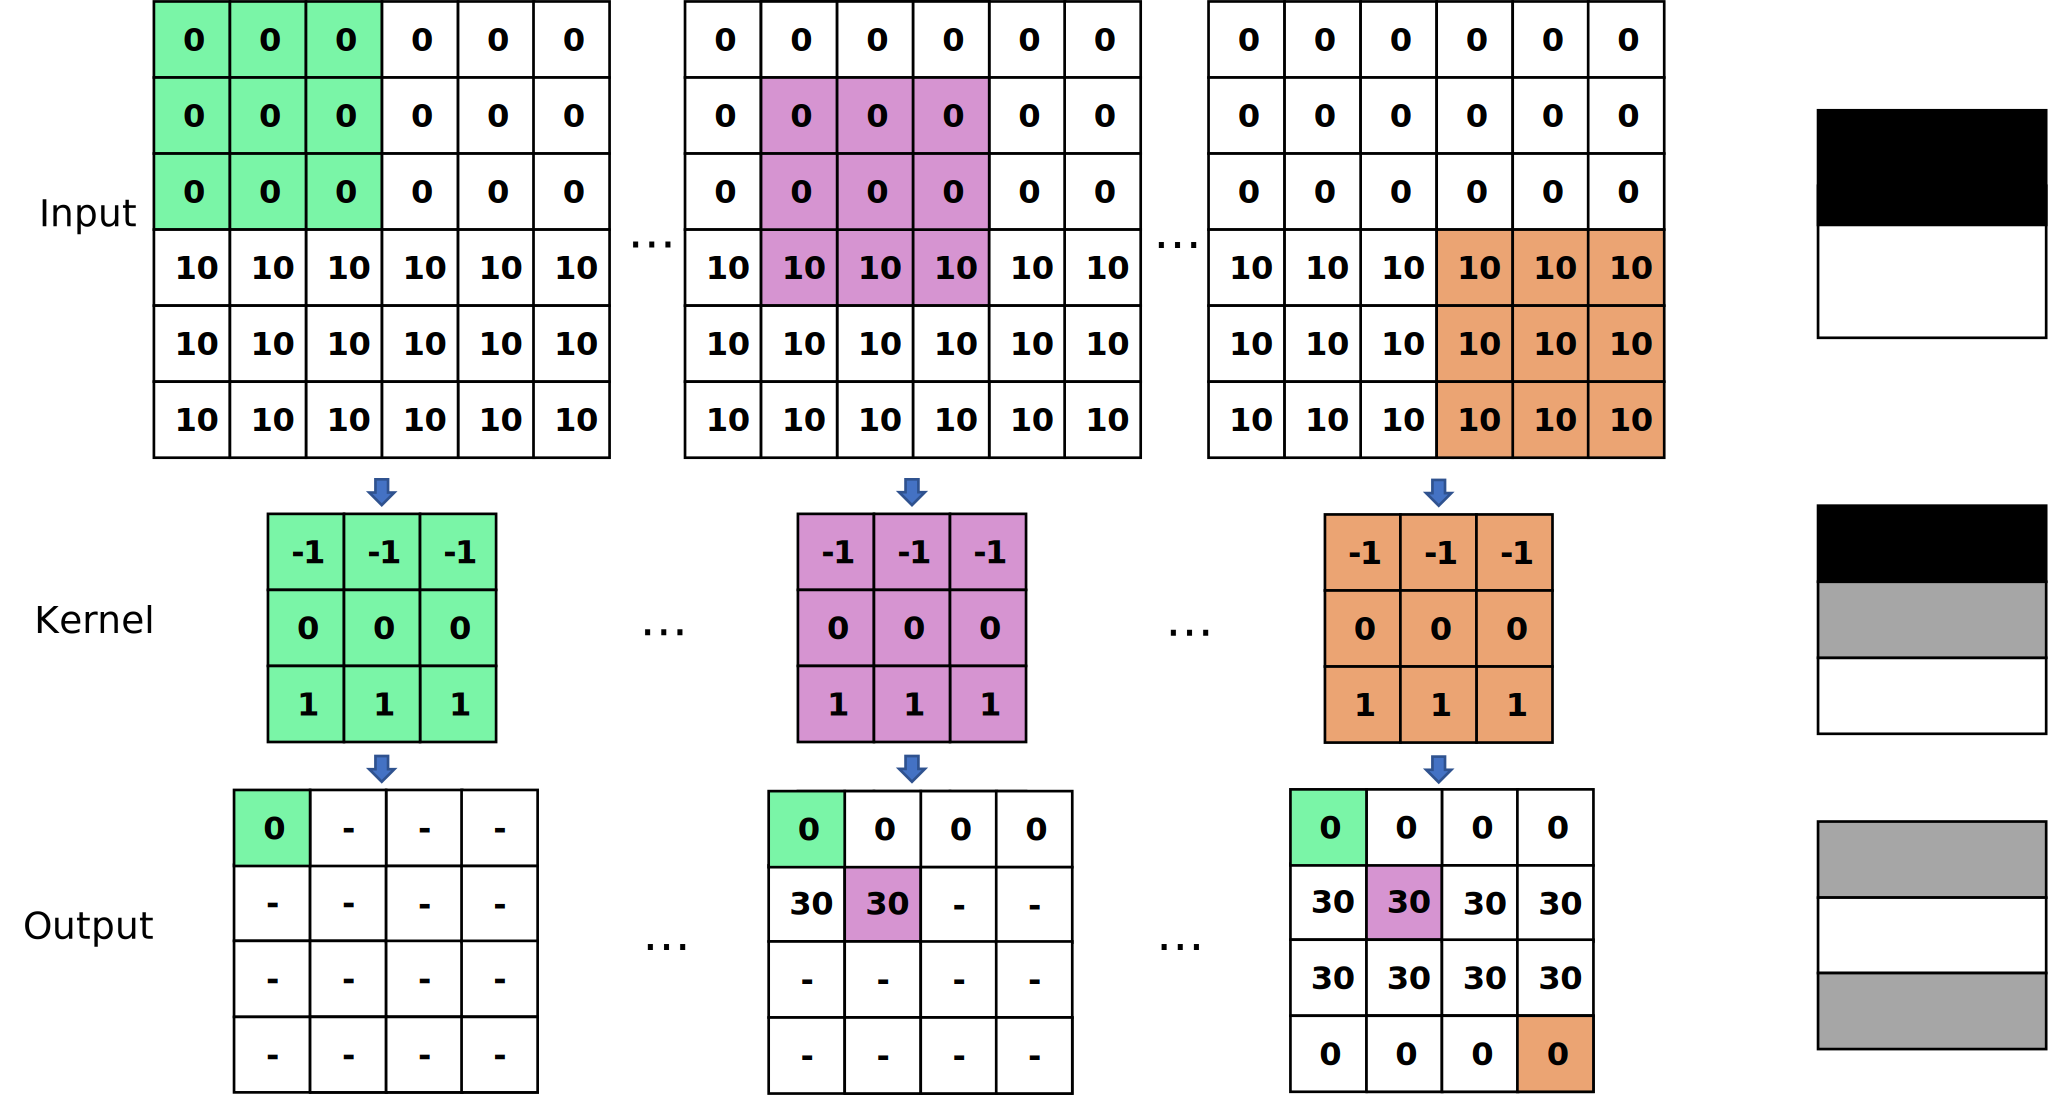
\includegraphics[scale=0.5]{figures/convolutions.png}
        \caption{Illustration of a \textit{valid} convolutional operation. The filter is applied repeatedly across the input. If the input had more channels, the filter would likewise have the equal depth. The size of input is 6x6, filter size is 3x3 and stride = 1. Resulting in the size of output being 4x4..}
      	\medskip 
        \label{convolutional_fig}
    \end{figure}
    
    \begin{figure}[H]
        \centering
        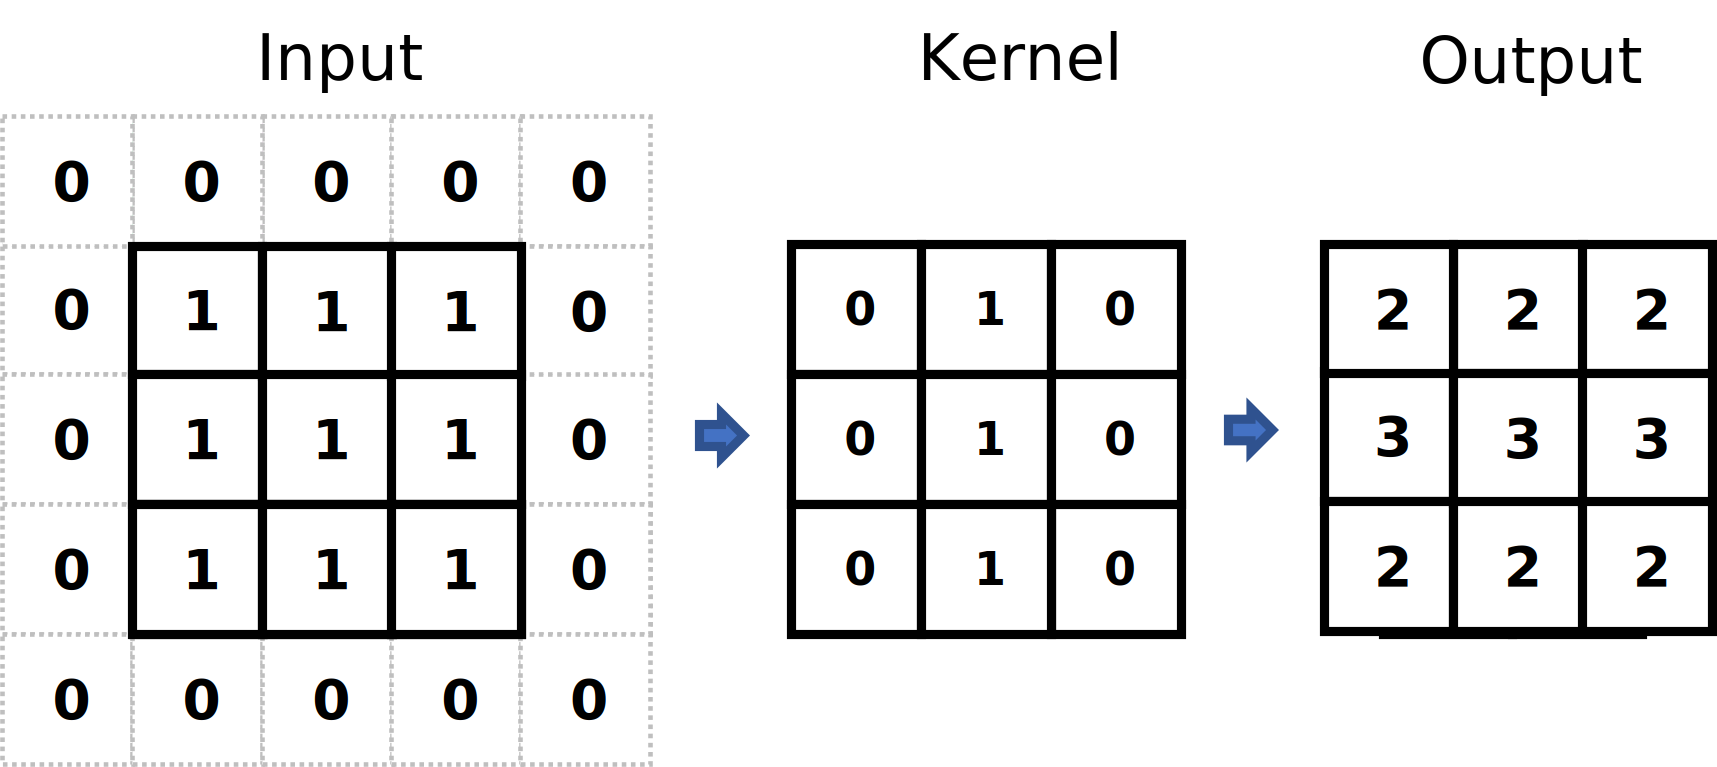
\includegraphics[scale=0.5]{figures/same_convolutions.png}
        \caption{Illustration of a \textit{same} convolutional operation. The size of the input is 3x3, but after padding the size is 5x5, filter size is 3x3 and stride is 1. Resulting in the size of output being 3x3, hence conserving the input size.}
      	\medskip 
        \label{same_convolutional_fig}
    \end{figure}
    

\subsection{Transpose convolutions}
    things
    
\subsection{Max-pool}
    \begin{figure}[H]
        \centering
        \includegraphics[scale=0.5]{figures/max_pool.png}
        \caption{Illustration of the max-pool operation with size = 2 and stride = 2.}
      	\medskip 
        \label{maxpool_fig}
    \end{figure}
    
    
\subsection{Convolutions through volumes}
    things
    
\subsection{Segmentation}
    Segmentation is a machine learning task where the objective is to assign one or several classification masks to the input\cite{He_2017_ICCV_segmentation}. This is again split into two different categories; \textit{semantic} and \textit{instance} segmentation. In semantic segmentation, you assign each pixel in the input to predefined classes. While in instance segmentation, you increase the complexity by applying semantic segmentation and thereafter assigning a bounding box to each individual object. Semantic segmentation is the variant used in this thesis, and an example can be viewed in figure \ref{segmentation_fig}.
    
    \begin{figure}[H]
        \centering
        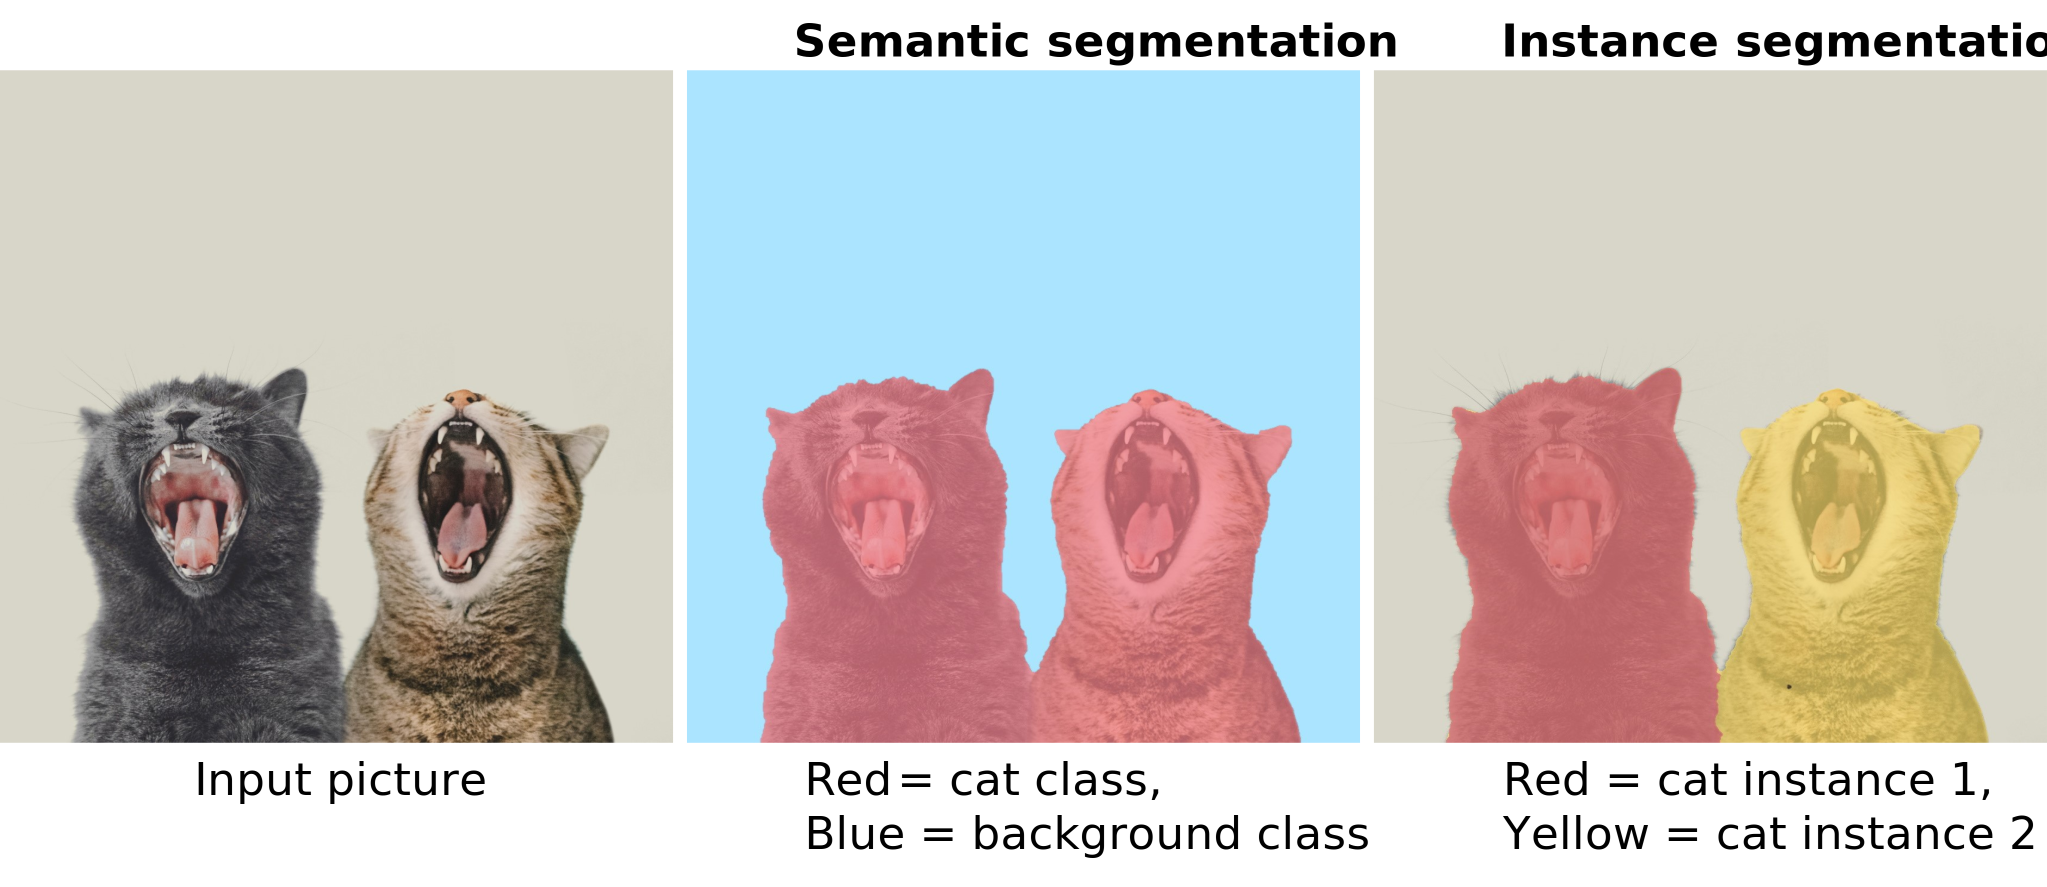
\includegraphics[scale=0.4]{figures/segmentation.png}
        \caption{Illustration of the difference between semantic and instance segmentation.}
      	\medskip 
        \label{segmentation_fig}
    \end{figure}
    
    

\section{U-Net}
    In this part I introduce the architecture of the deep learning \gls{ann} used in this thesis called U-Net. This is a fully convolutional state-of-the-art\cite{rajak2021segmentation} semantic segmentation \gls{ann} and was initially developed for biomedical use by \citeauthor{unet_ronneberger2015}\cite{unet_ronneberger2015}. The \gls{crimac} used this model in their project (described in \ref{unet_paper_acoustic}) and had to do some small modifications to the network to fit their task. This modified U-Net is the one presented in this section, as this is the one used in the experiments. The core functionality of the network stays true to the original Unet and the alterations done will be explained later in this section.
    
    \begin{figure}[H]
        \centering
        \includegraphics[scale=0.5]{figures/unet_arrows.png}
        \caption{U-Net architecture, the downwards facing arrow illustrates the contracting path and the one facing upwards is the expanding path.}
      	\medskip 
        \label{unet_fig}
        \hspace*{15pt}\hbox{\scriptsize Credit: \citeauthor{brautaset2020acoustic}\cite{brautaset2020acoustic}}
    \end{figure}
    
    Unet utilized what \citeauthor{unet_ronneberger2015}\cite{unet_ronneberger2015} called a contracting path to identify what was in a picture, while an expanding path to localize where it was. These two branches were symmetrical, and together they formed a U-shape, giving the network its name. The contracting path can be looked at as five different stages of processing, from top to bottom, in figure \ref{unet_fig}. Each stage applied the same operations to its given input. For each stage, this consisted first of two 3x3 same convolutions with their individual ReLu activation functions. Initially, the feature channels would be increased to 64, and later doubled for each contracting stage. The convolutions were followed by a 2x2 max pooling operation with stride 2 to decrease the resolution of the output from the convolutional operations, and then send this feature map down to the next stage. At the bottom stage, the only things that changed was the use of transpose convolutions instead of max pooling to now increase the resolution. At each subsequent stage going back up the expanding path, the number of feature channels were halved. To aid the localization, the output of the previous stage would be concatenated with the output feature map of a stage from the contracting path with the same size. At the last stage, when the resolution had reached it original size, a 1x1 convolution was applied instead of increasing the resolution. The 1x1 convolution mapped the 64 feature channels to the 3 classes. The softmax was then calculated between these classes, giving each pixel a value between [0,1], summarized over all classes to 1. Hence, giving you a segmentation map of each class with the same size as the input. In this thesis, this will be a semantic segmentation of the classes \textit{background}, \textit{other } and most importantly \textit{sandeel}.
    
    Here I list the changes from \citeauthor{unet_ronneberger2015}s original U'net performed in article \ref{unet_paper_acoustic}. Firstly, minor changes were made to adapt U-net to the acoustic data, as the input now had the form 4 x 256 x 256. The four channels being the frequencies used. The convolutions were as mentioned in the previous paragraph set to \textit{same} instead of \textit{valid}, as were the original setting. This was done to make the size of the input and output match. Further, batch normalization was added to each convolution. 
    
    




\section{The data and tools}
    The data was provided by the \gls{imr} and I had access to a broad selection of yearly trawl cruises spanning from 2011 to 2020. In this chapter, I will delve into the data itself to give you a clearer picture of how it looked, how I acquired it and what tools I utilized.
    
    \subsection{The data provided (.RAW)}
        The files were initially presented to me as ".RAW" \cite{raw} and ".WORK" files. ".RAW" is the uncompressed raw output from the echo sounder. The same format is used by cameras before they are converted to, for example, ".JPEG". Because they are uncompressed, they do not lose any data. Unfortunately, this also makes them large. The ".WORK" files are the annotations of the ".RAW" files done by operators using a system called the \Gls{lsss}\cite{lsss}. The data from 2020 alone which spanned three months took 240 GB of storage space and stored on a remote server.
        
        SJEKK DATAEKSEMPEL!
    \subsection{Windows Azure}
        Windows Azure \cite{azure} is a platform owned by Microsoft that provides cloud solutions for several services. My use was to access a remote storage provided by the \gls{imr} and mount this to my local computer. Thus enabling me to download the data for this thesis from \gls{imr}s server. 
    
    \subsection{Docker}
        Docker \cite{docker} is an open source platform that provides what they call containerization and is owned by the company under the same name, Docker, Inc. If you are familiar with virtual machines, then containerization will be very familiar to you. Docker is based on the Linux kernel, and enables you to create a container, which is an independent process that uses resources from the main instance. For each container, you can manage its own dependencies like programming languages and libraries. These containers can then be shared with others as images files, and as they can be run without the receiver having to manage the aforementioned dependencies as this is built into the image. Thus, you can make an application or code easily accessible for other people, as long as they have installed Docker.
        
    \subsection{Zarr}
        By using the ".ZARR" \cite{zarr} format, you gain access to store chunked compressed  multidimensional arrays. There are several highlights from this library, but I used primarily the ability to access the arrays on disk. This means I did not need to load the entire array into memory and could work with the array and access parts of it without hardware limitations.
        
    \subsection{CRIMAC-pipeline} \label{CRIMAC-pipeline}
        Together, the \gls{nr} and the \gls{imr} developed a pipeline\cite{crimac_pipeline} to classify the acoustic backscatter in echo sounder data. This was part of the work described earlier in \ref{unet_paper_acoustic} and is accessed by using docker. They also provide the image for a container to access the data through Azure.
        
        The pipeline is run using one docker container, which in turn downloads and runs four others:

            \begin{description}
              \item[$\bullet$ Preprocessor] Preprocesses the ".RAW" and ".WORK" to respectively ".ZARR" and ".PARQUET" files. Since frequencies can have different resolutions, all are re-gridded to the 38kHz frequency.
              \item[$\bullet$ Unet] Using a pretrained deep learning model called Unet it produces pixel based annotations
              \item[$\bullet$ Bottom detection] Identifies the bottom and generates a pixel based map stored as ".ZARR".
              \item[$\bullet$ Report generation] Takes in the output from the bottom detection, Unet and the preprocessed ".RAW" file and generates a report for the \gls{ices}.
    
            \end{description}

        The Unet, bottom detection and preprocessing is the same as described in section \ref{unet_paper_acoustic}.

    \subsection{Xarray}
        Xarray\cite{xarray} is a Python package that is made for working with multidimensional arrays. It is based on NumPy and adds labels in the form of attributes and coordinates on top of the NumPy-arrays. This was the library I used for accessing and working more efficiently with the ".ZARR" arrays, as I was already very familiar with NumPy.
        
        
    \subsection{Pytorch} \label{Pytorch}
    
    